\section*{Farina et all (1997, Capítulo 3): Economia dos custos de transação}

A partir da NEI e do conceito de custos de transação, a forma de organização se torna uma \textbf{variável endógena}, ou seja, uma variável de escolha. Com isso, é possível entender a reestruturação de sistemas produtivos dadas mudanças no ambiente institucional.

\subsection*{Pressupostos comportamentais}

Para a existência de custos de transação, é preciso pressupor:

\begin{description}
	\item[Racionalidade limitada:] Contratos são necessariamente incompletos
	\item[Comportamento oportunista:] Renegociação entre as partes é inevitável
\end{description}

\subsubsection*{Racionalidade ilimitada}

Seguindo Williamson, os autores apresentam três níveis de racionalidade:

\begin{description}
	\item[Forte:] Agentes são capazes de absorver e processar toda a informação disponível e agir de forma otimizadora
	\item[Limitada (semiforte)] Agentes agem racionalmente, mas de forma limitada de modo que tomam decisões \textbf{satisfatórias} e incluem salvaguardas nos contratos dada a inevitável incompletude dos acordos entre as partes. Uma vez que a racionalidade é um \textbf{recurso escasso}, geram custos associados a sua utilização.
	\item[Procedural] Racionalidade dos agentes é \textbf{insuficiente} para direcionar a escolha de um quadro institucional. Como consequência, adotam \textbf{rotinas} para enfrentar as contingências.
\end{description}

Em seguida, distinguem racionalidade limitada de \textbf{incerteza}. Resumidamente, o primeiro é uma característica do indivíduo enquanto o seguindo é do \textbf{ambiente}.
Adiante, demarcam as diferenças da NEI da \textbf{teoria dos contratos} em que os custos podem ser identificáveis \textit{\textbf{ex ante}} na última abordagem enquanto a NEI parte da impossibilidade  de considerar os custos em sua totalidade na elaboração dos contratos.

\subsubsection*{Oportunismo}

Ainda partindo de Williamson, os autores identificam três níveis de comportamento auto-centrado:

\begin{description}
	\item[Oportunismo] Não há restrição aos comportamento egoísta tanto \textit{ex-ante} quanto \textit{ex-post}
	\item[Sem oportunismo] Acordos serão mantidos durante a execução do contrato. Usual e implicitamente, assume-se que a utilização do \textbf{aparato judicial} é precisa, sem custos e instantânea.
	\item[Ausência de auto-interesse] Ações individuais não são comandadas pelos próprios indivíduos, mas sim, por uma entidade externa à eles (ex: ideologia)
\end{description}

Os autores argumentam que pressupor um comportamento oportunista não implica pressupor ausência de ética, mas sim que a ética é uma instituição (informal) que visa restringir o comportamento oportunista. Seguindo Williamson, pontuam que as estruturas de governança são modeladas de modo a impedir o comportamento oportunista de uma das partes.

\subsection*{Dimensão das transações}

Em linhas gerais, a diversidade dos \textbf{tipos de contratos} está associada à \textbf{dimensão de cada transação} de modo que os custos de transação são uma função destes atributos (dada a estrutura de governança).

\subsubsection*{Especificidade dos ativos}

Ativos específicos são aqueles que se não empregados na função a que foram designados, perdem valor significativamente e depende da continuidade da transação à qual ele é específico. Sendo assim, a especificidade dos ativos não pode ser desassociada do tempo. Consequentemente, quando empregados na transação à qual são específicos, geram uma \textbf{quase-renda} de modo que tal transação pode ser configurada como um monopólio bi-lateral.
Adiante, os autores distinguem especificidade de \textit{sunk costs} e custo fixo. Em seguida, são apresentados os tipos de especificidade dos ativos:

\begin{itemize}
	\item Locacional
	\item Ativos físicos
	\item Ativos humanos
	\item Ativos dedicados
	\item Marca
	\item Temporal
\end{itemize}

\subsubsection*{Frequência}

Resumidamente, a frequência de uma transação é relevante para a escolha de um \textbf{estrutura de governança} adequada à essa transação e tal importância se manifesta em dois aspectos:

\begin{itemize}
	\item Diluição dos custos da adoção de um mecanismo completo
	\item Possibilidade de construção de reputação
\end{itemize}

Além disso, pontuam que uma única transação não é suficiente para a elaboração de uma estrutura de governança de modo que é realizada através do mercado \textit{spot}. Também destacam que a repetição de uma transação só se traduzirá em reputação se a economia  dos custos de transação forem maiores que o aumento dos custos de transformação. A relevância da frequência se dá pela elevação dos custos associados ao comportamento oportunista (desde que este seja observável).

\subsubsection*{Incerteza}

Os autores discutem os diferentes tipos de incerteza. Vale pontuar que esta dimensão é relevante por explicitar os limites da racionalidade e incompletude dos contratos.

\subsection*{Um modelo para a escolha da forma organizacional}

Ao longo desta seção, são apresentados dois modelos para a \textbf{escolha da forma organizacional} mais pertinente a uma transação, comparando a \textbf{eficiência relativa} de cada tipo de governança:

\begin{description}
	\item[Williansom (1991)] Eficiência das formas organizacionais é função das especificidades dos ativos
	\item[Riordan e Willianson (1985)] Incorpora os custos de transação aos custos de transformação (ortodoxo)
\end{description}
Vale destacar que ao comparar a eficiência relativa e não absoluta, tal abordagem dispensa a necessidade de se calcular os \textbf{custos de transação} em termos absolutos. Além disso, as demais dimensões das transações são tratadas como deslocamentos da especifidade dos ativos. As estrutura de governança (mercado, verticalização e híbrido) se distinguem pelo \textit{trade-off} entre \textbf{incentivo e controle}. A comparação entre hierarquia e mercado se dá em três níveis:

\begin{description}
	\item[Tecnológico] Mercado é mais eficiente que a hierarquia por se aproveitar mais das economias de escala estáticas, economias de escopo e benefícios da agregação de demandas não-correlacionadas
	\item[Estrutura de informação] Na forma hierárquica, as informação privativas passam a ser comuns. Em outras palavras, a estrutura de informação é diferente para cada estrutura de governança. Supõe-se que o mecanismo de mercado é mais eficiente
	\item[Organizacional] Diz respeito à \textbf{natureza dos contratos} de cada forma organizacional e é nesta distinção que reside o \textit{trade-off} entre incentivo e controle. O mercado apresenta incentivos fortes (associados a relação entre esforço e remuneração) e pouco controle. A forma hierárquica possui um maior controle porque as questões jurídicas podem se resolver internamente.
\end{description}

Uma vez que a \textbf{adaptação} das instituições são fundamentais para NEI, Willianson as separa em autônomas e cooperativas. Na primeira, os preços são suficientes para a escolha de adaptações e é mais eficiente por estar mais próxima da fonte da perturbação. Na segunda, diz respeito à presença de uma dependência bilateral entre as partes, de modo que é necessário um mecanismo que induza a cooperação. Vale relembrar que uma adaptação inadequada implica custos de transações mais elevados. Resumidamente, o mercado é mais eficiente na implementação de adaptações autônomas enquanto a hierarquia é mais eficiente na adaptação cooperativa.
Os modelos apresentados destacam que incentivo e controle são mais ou menos importantes a depender da \textbf{especificidade dos ativos}.
Por fim, a partir da distinção entre as estruturas de governança, conclui-se que não é possível desenvolver uma forma organizacional que proporcione simultaneamente o controle da hierarquia e o incentivo fortes do mercado.

\paragraph*{Modelo: forma reduzida}

Os custos de governança do mercado ($M$), da forma híbrida ($X$) e da hierarquia ($H$) são representados em função da especificidades dos ativos ($k$) e de um vetor de descolamento ($theta$):

$$
M(k, \theta) \hspace{1cm} X(k, \theta) \hspace{1cm} H(k, \theta)
$$
são impostas as seguintes restrições

$$
M(0, \theta) < X(0, \theta) < H(0, \theta) \forall \theta \in R^n
$$
ou seja, na ausência de especificidade dos ativo, o mercado é a forma organizacional mais eficiente enquanto a necessidade de controle aumenta com a especificidade dos ativos

$$
M' > X' > H' \forall \delta k
$$

\begin{figure}[h]
	\centering
	\caption{Especificidade dos ativos e estrutura de governança}
	\label{fig:screenshot002}
	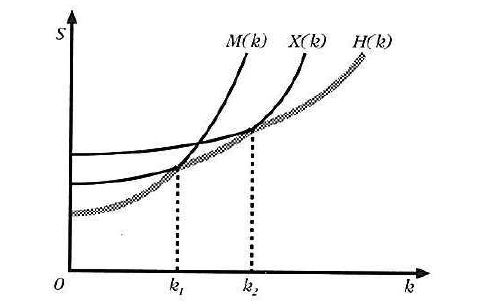
\includegraphics[width=0.7\linewidth]{screenshot002}
\end{figure}


\paragraph*{A transformação fundamental}

\begin{description}
	\item[Definição:] Diminuição do número de transacionistas potencias \textit{ex-post}. Como consequência, são criados instrumentos contratuais para lidar com as contingências desta transformação. A concorrência deixa de ser um indicador \textbf{suficiente} de eficiência.
\end{description}

\paragraph*{Modelo principal}

\subparagraph*{Tecnologia e produção comum}

Como simplificação temporária, considera-se que a produção independe da forma organizacional. Desse modo, as receitas e os custos de transformação são os mesmos

$$
R = R(Q)
$$

$$
C = C(Q, k, \theta^{-})
$$
em que $Q$ é a quantidade produzida, $k$ é a já mencionada especificidade dos ativos e $\theta^{-}$ é um parâmetro de descolamento que implica em menores custos de transformação. Com isso é possível determinar a função de lucros como

$$
\pi^*(Q,k, \theta^{-}) = R(Q) - C(Q, k, \theta^{-}) - \gamma k
$$
Conclui-se que a receita marginal da especificidade deve-se igualar ao seu custo marginal e que as variáveis decisórias que maximizam o lucro ($Q^*$ e $k^*$) são obtidas pela condição de primeira ordem. Em seguida, na presença de custos de governança, as formas organizacionais se distinguem 

$$
G^M = V^M(k)
$$
$$
G^X = \beta^X  + V^X(k)
$$
$$
G^H = \beta^H  + V^H(k)
$$
com
$$
\beta^H > \beta^X > 0 \hspace{1cm} V^M > V^X > V^H > 0
$$
Em resumo, na ausência de ativos específicos, o mercado é a estrutura mais eficiente. No entanto, na medida que tal especificidade aumenta, o mercado apresenta maiores custos relativamente. O nível ótimo de especificidade dos ativos é dado pelos custos de governança e o componente de custos de transformação que depende da especificidade.
Este nível ótimo, por sua vez, é distinto para cada forma organizacional. Além disso, quanto maior a especificidade dos ativos, maior a produção ótima da forma hierárquica em relação a uma estrutura com mais incentivos.

\subparagraph*{Tecnologia de produção distinta}

Nesta versão, a tecnologia de produção varia com a forma de governança e reforçam os resultados anteriores: formas organizacionais com maior controle são menos prejudicadas à medida que aumenta nível de produto e de especificidade. No entanto, na medida que o produto e a especificidade tendem ao infinito, a diferença entre as formas organizacionais tende à zero.
Além disso, firmas maiores e mais verticais se aproveitam de economias de escala e assim reduzem os custos de \textbf{transformação}.
Por fim, destacam que mesmo que o grau de verticalização seja diretamente proporcional à especificidade dos ativos, nada garante que maior especificidade gera maiores custos de transação em termos absolutos (apenas relativamente mais eficiente).


\begin{sigstatement}
\sffamily
\mdfdefinestyle{stylesigstyle}{linewidth=0.7pt,
backgroundcolor=styleblueback,linecolor=stylebluetext,
fontcolor=stylebluetext,innertopmargin=6pt,innerrightmargin=6pt,
innerbottommargin=6pt,innerleftmargin=6pt}
{%	
\begin{mdframed}[style=stylesigstyle]%
	
\section*{Dúvida}%

\begin{itemize}
	\item Existe uma precedência entre incompletude dos contratos e oportunismo? Ou melhor, os contratos incompletos induzem comportamentos oportunistas ou são incompletos por que os agentes são oportunistas?
	\item Em que medida as conclusões do modelo do Williamson são sensíveis às hipóteses de eficiência adotadas?
	\item Como tratar de bens públicos nesse modelo?
	\item A NEI parte da racionalidade limitada para destacar a relevância e incompletude dos contratos. No entanto, ao apresentar o modelo de Williansom são mostradas as condições de maximização de lucros. Este comportamento otimizador não está em conflito com a hipótese de racionalidade limitada? É razoável supor que são maximizadores na produção mas não na elaboração de contratos?
	\item Ao apresentarem o modelo mais simplificado de Riordan e Williamson, afirmam (p.~106): `` O nível ótimo de especificidade dos ativos é dado pelos custos de governança e o componente de custos de transformação que depende da especificidade. '' No entanto, a especificidade é uma variável endógena ou exógena à forma organizacional? Firmas são capazes de escolher quão específico são seus ativos para realizar a produção?
\end{itemize}

\end{mdframed}}
\end{sigstatement}